\section{Planning Algorithm}
\label{sec:PlaniAlg}


\subsection{STRIPS Algorithm}
The implementation is based on the STRIPS algorithm which works in the following way:

The STRIPS is provided with an initial state, a final state (containing the goals of the problem) and a set of operators. We use a simplified version of STRIPS where the goal state cannot state predicates that need to be false - it can only specify a conjunction of predicates that need to be true in the end.

The STRIPS algorithm uses a stack that can contain single predicates, lists of predicates and operators to calculate a plan of operators that reach the final state starting from the initial state. 

A pseudo-code example of the STRIPS algorithm can be found in listing \ref{code:strips}.

\begin{lstlisting}[language=Java, 
	caption=The STRIPS algorithm, 
	keywordstyle=\color{blue},
	stringstyle=\color{red},
	commentstyle=\color{magenta},
	label = {code:strips}]
State initialState, finalState
State currentState = initialState;
List<Operator> operators;
Stack stack;
List<Operator> plan;

stack.push(finalState.predicateList);
for(predicate : finalState.predicateList):
   stack.push(predicate);

while(!stack.isEmpty()):
   element = stack.pop();
   
   case element instanceof Operator:
      currentState.apply(element);
      plan.add(element);
   
   case element instanceof List<Predicate>:
      for(predicate : element):
         if predicate not true in currentState:
            stack.push(predicate);
   
   case element instanceof Predicate:
      if element.isFullyInstantiated():
         if element not true in currentState:
            operator = findOperatorToResolve(element);
            stack.push(operator);
            stack.push(operator.preconditions);
            for(predicate : operator.preconditions):
               stack.push(predicate);
         else: 
            // Look for constant c to instantiate element.
            // Set c in entire stack.
            instantiate(element);

return plan;
\end{lstlisting}

\subsection{Heuristics}
\label{subsub:heuristics}

In our specific implementation of the STRIPS algorithm to solve the coffee problem, we use two different heuristics to reduce the number of steps $x$ that are needed to achieve the final state. These heuristics determine in which order the predicates belonging to a list of predicates get pushed onto the stack, and which constant is selected out of several options when instantiating the predicates.

\subsubsection{The Served-Heuristic}

The Served-Heuristics determines in which order the robot processes the different petitions to serve the coffee. If the petitions are processed in a random order or simply based on their position in the description of the world, the robot is likely to make a lot of unnecessary steps. The optimal solution here belongs to the class of the Traveling Salesman Problem and is too complex to exactly compute for a large number of petitions.

In our implementation we resorted to the nearest-neighbor heuristic (NN-heuristic) to get a good solution for this problem with relatively little computational effort. The steps of this algorithm are the following:

\begin{enumerate}
	\item Start at the beginning position of the robot.
	\item Find shortest distance between current position and an unvisited Served predicate $S^*$.
	\item Save $S^*$ to sequence and set current position to $S^*$.
	\item Mark $S^*$ as visited.
	\item If all Served predicates are visited, terminate
	\item Go to step 2.
\end{enumerate} 

The difference between visiting petitions in their order (from $P_1$ to $P_4$) or choosing a path based on the NN-heuristic can be seen in figure \ref{fig:1}. While the the path based on the petition number requires 21 steps, the NN-heuristic only requires 17 steps. Empirical results of the NN-heuristic can be found in section \ref{sec:results}.

\begin{figure}[!ht]
\centering     %%% not \center
\subfigure[21 steps with petition number order]{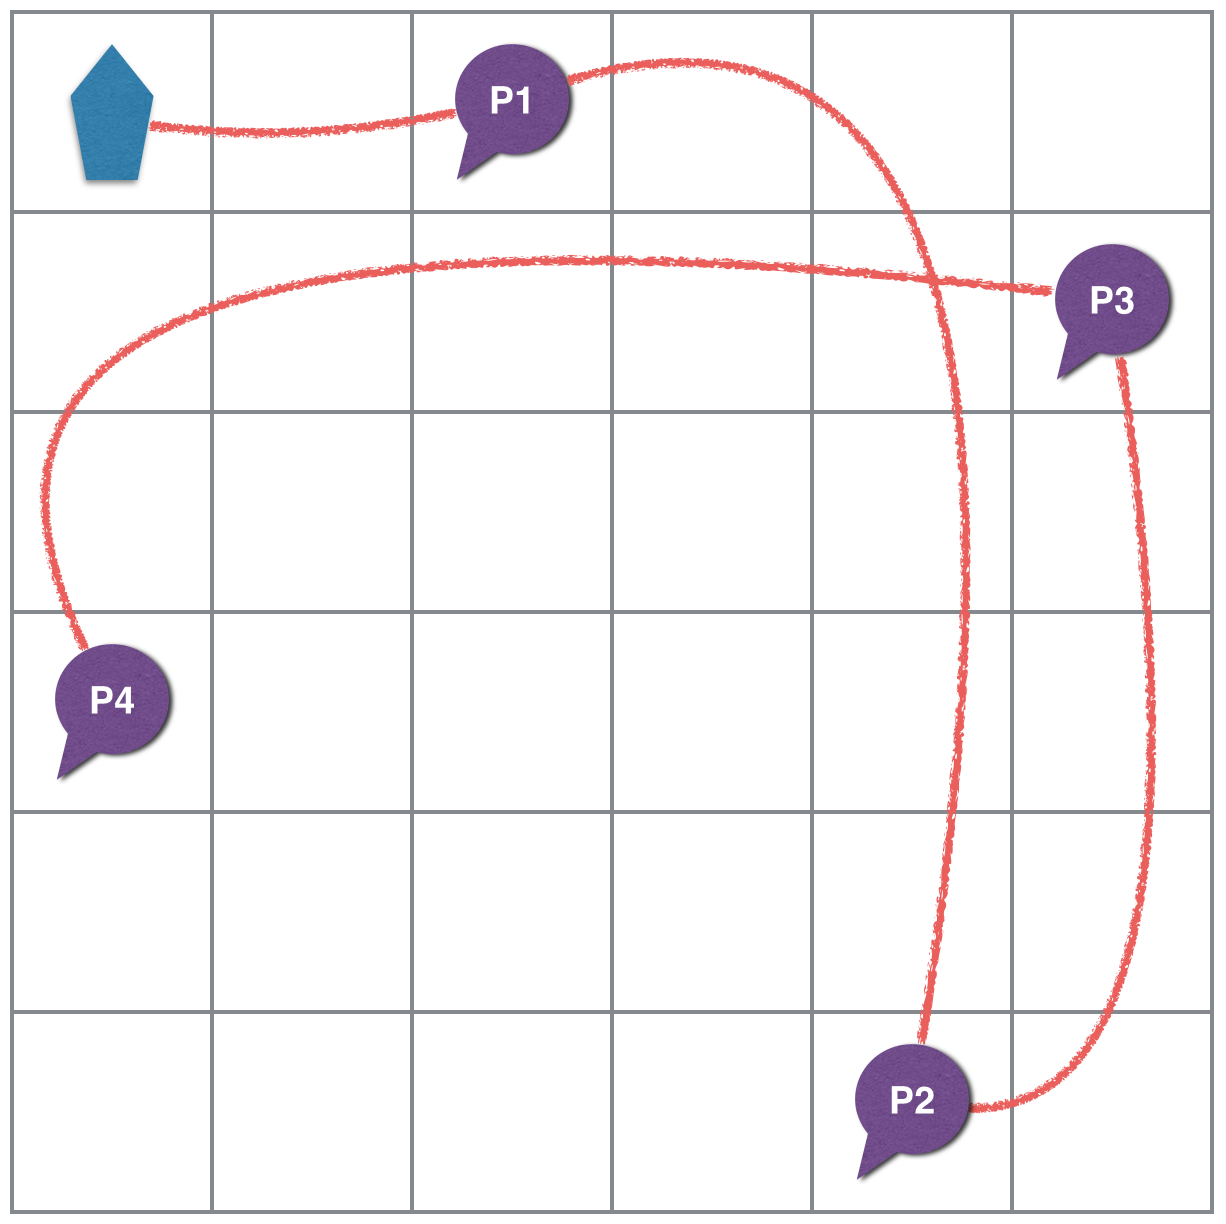
\includegraphics[width=60mm]{img/servedHeur1}}
\subfigure[17 steps with NN-heuristic]{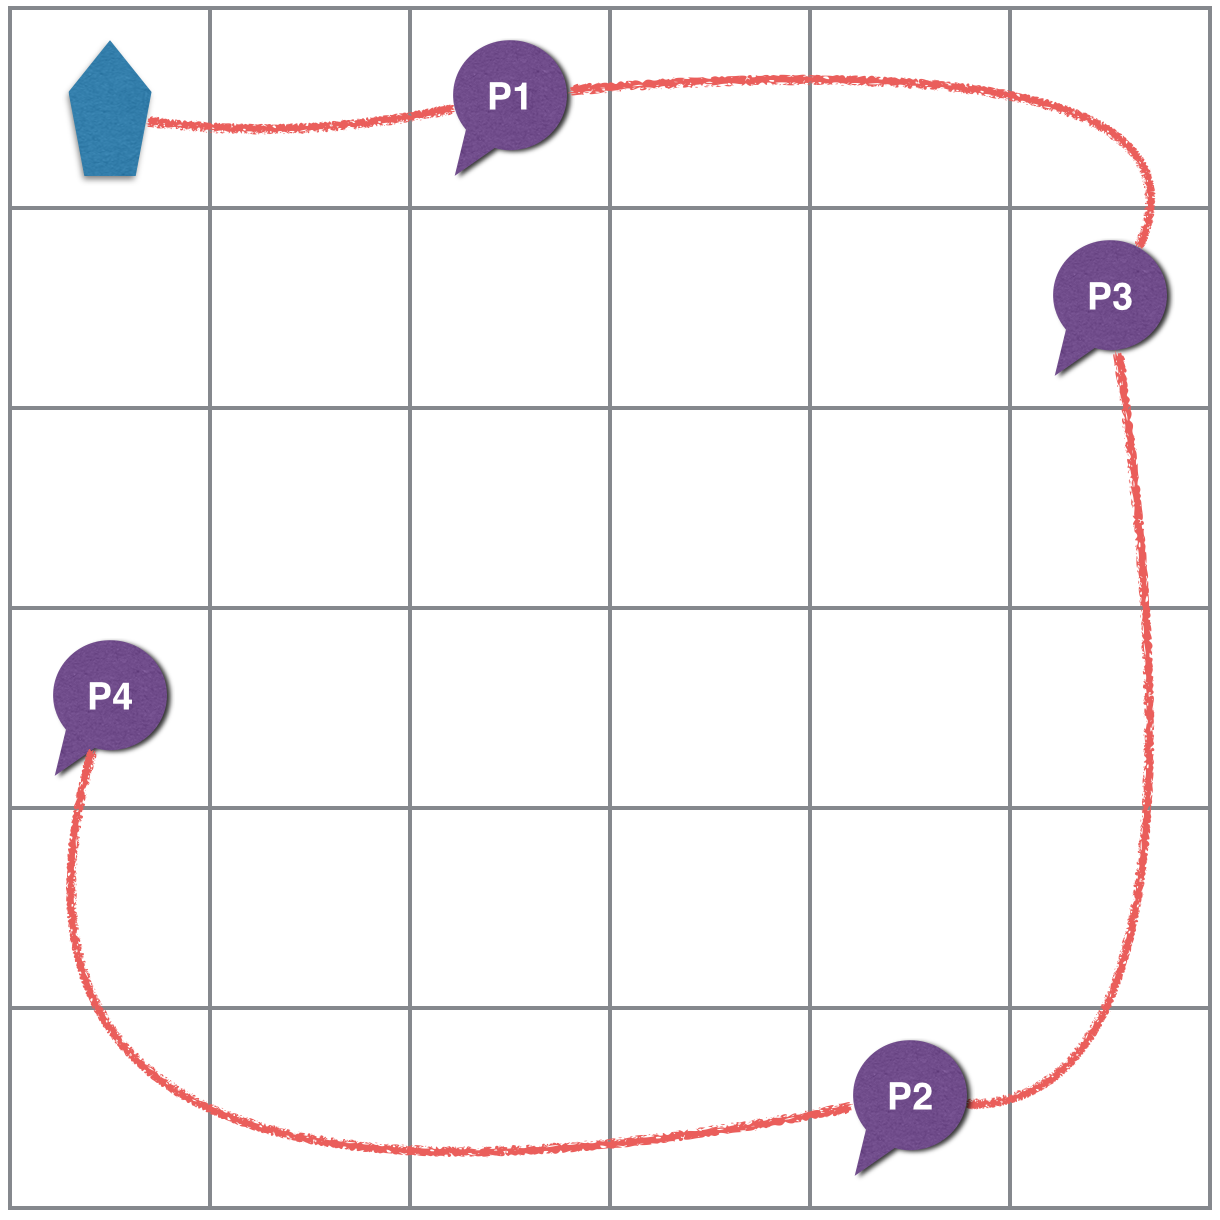
\includegraphics[width=60mm]{img/servedHeur2}}
\caption{Petition Number Order vs. NN-Heuristic}
\label{fig:1}
\end{figure}



\subsubsection{The Machine-Heuristic}

When planning to serve coffee for a specific petition, the planner has to find a suitable machine that can brew the fitting number of cups. In some worlds there might be more than one possible Machine predicate with a fitting $n$. The right choice of machine is focus of our second heuristic.

Without using a heuristic, STRIPS instantiates with an arbitrary compatible machine, which can lead to big detours (as shown in example (a) of figure \ref{fig:2}). A first improvement of the number of steps can be achieved by choosing the machine that is closest to the current position of the robot, as in example (b) of figure \ref{fig:2}. 

In our heuristic we don't only consider the distance between current position and the machine, but also the distance from that machine to the next petition. For the robot position $r$, the machine position $m$ and the petition location $p$, the distance is calculated as:

$heurDist(m)  = dist(r, m) + dist(m, p)$

We then choose the machine $m$ with the smallest $heurDist(m)$.

\begin{figure}[!ht]
\centering     %%% not \center
\subfigure[First machine]{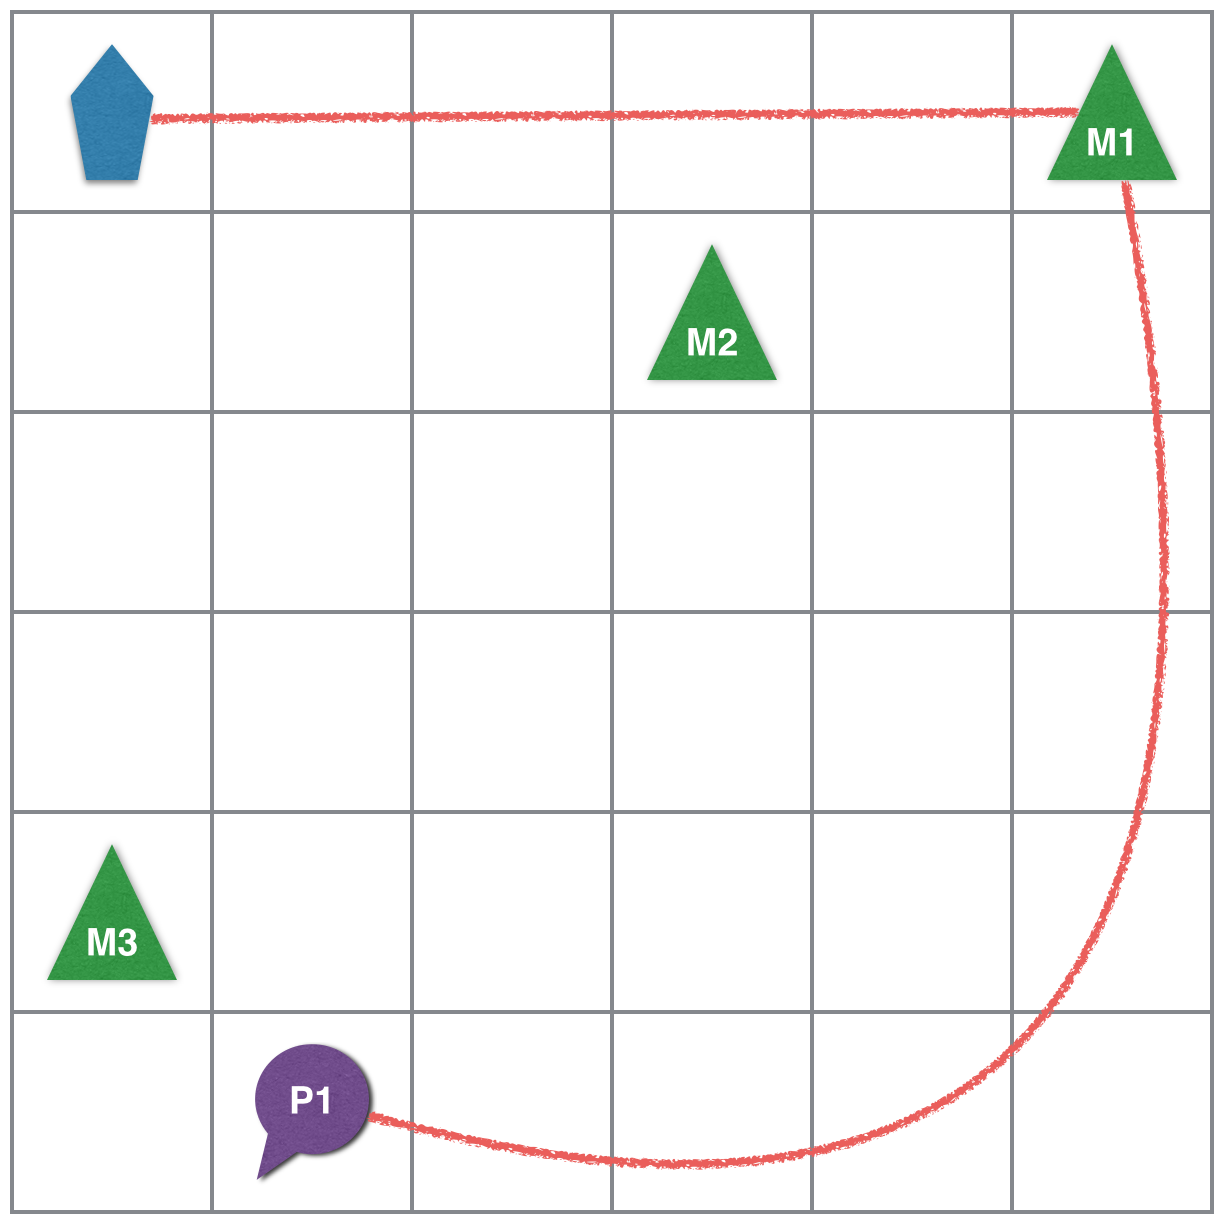
\includegraphics[width=40mm]{img/mHeur1}}
\subfigure[Nearest machine]{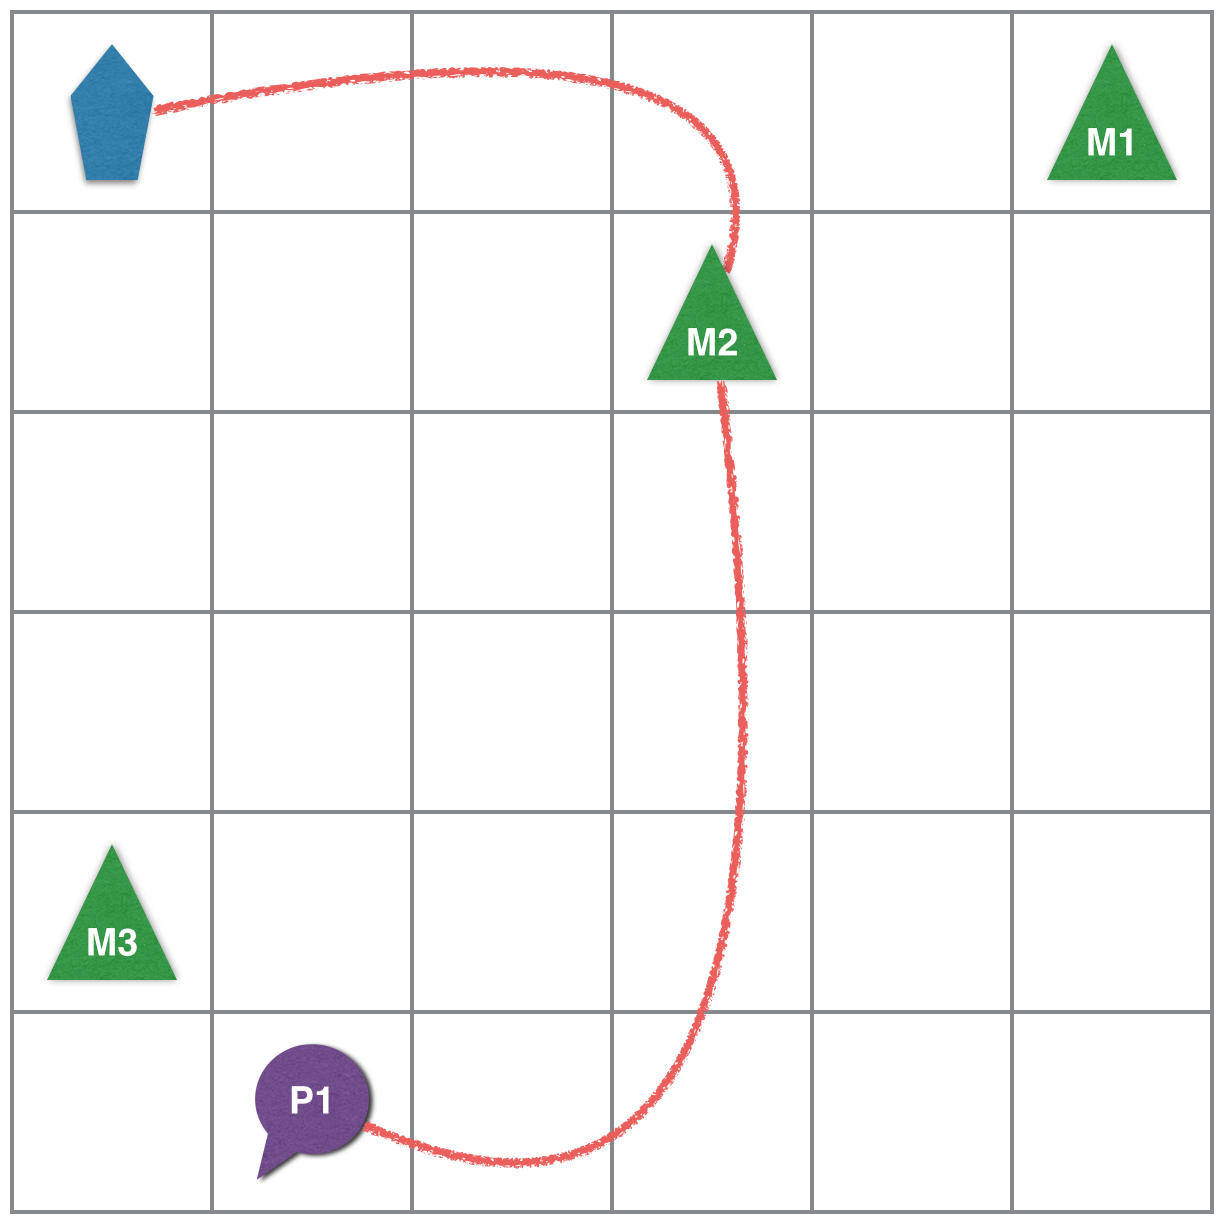
\includegraphics[width=40mm]{img/mHeur2}}
\subfigure[Best total distance]{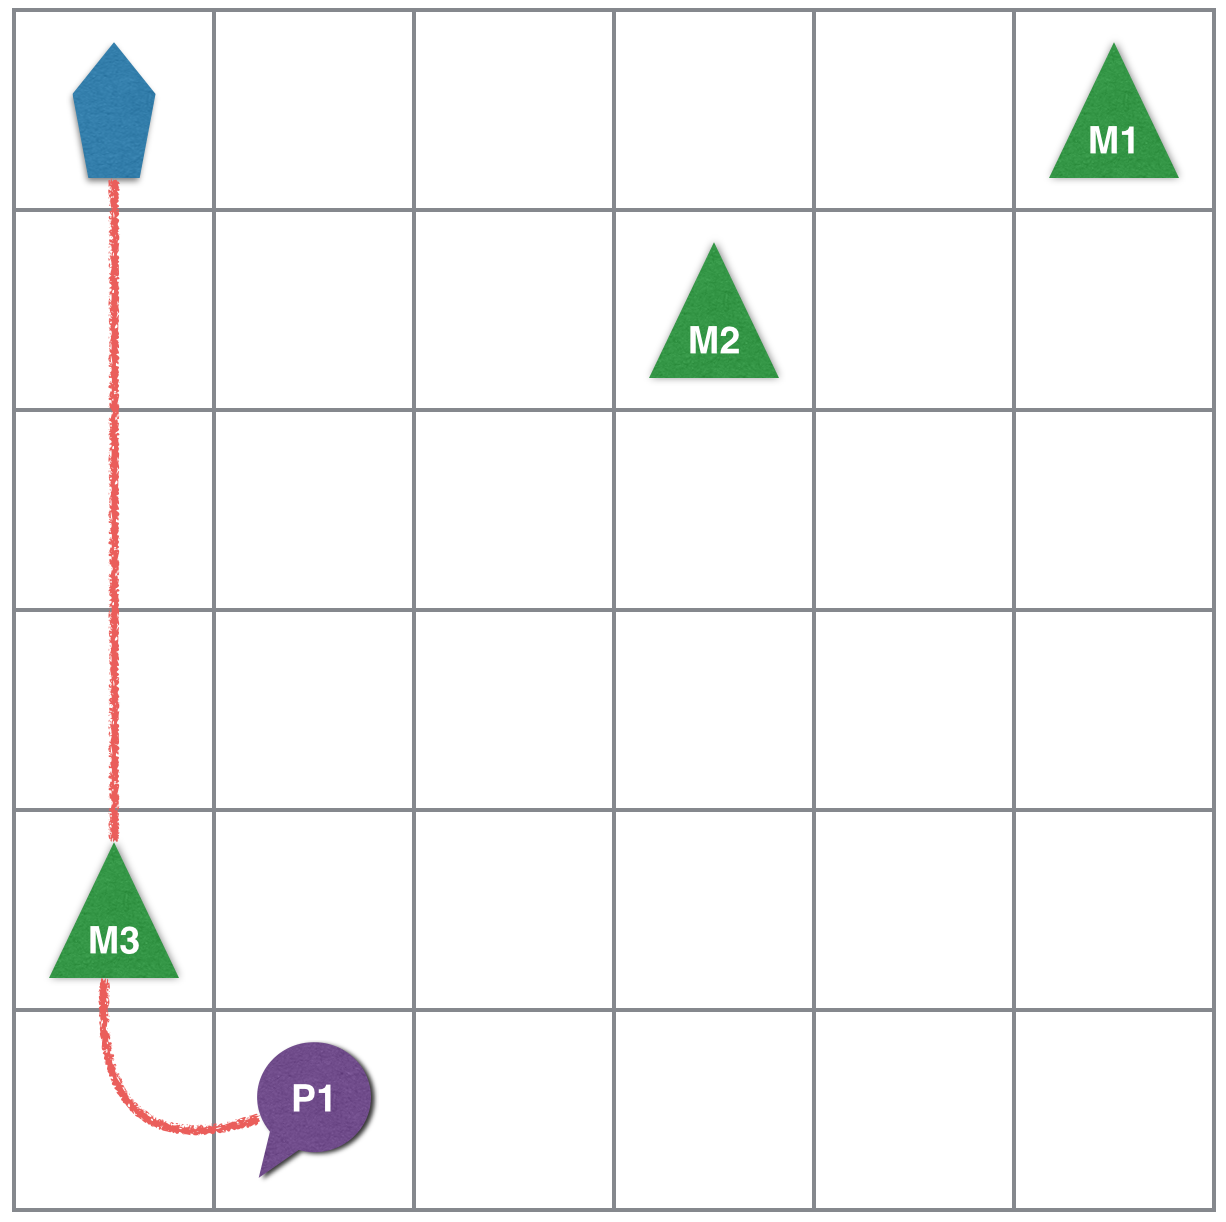
\includegraphics[width=40mm]{img/mHeur3}}
\caption{Comparison of Machine Selection}
\label{fig:2}
\end{figure}

Empirical results of this heuristic can be 

